\section{Модификация проекта «Изображение проекции полиэдра»}
\subsection{Постановка задачи}

Модифицируйте эталонный проект таким образом, чтобы определялась и печаталась следующая характеристика полиэдра: сумма длин проекций полностью невидимых рёбер, центр которых находится на расстоянии строго меньше $1$ от плоскости $x=2$.

При выполнении задания должна использоваться следующая трактовка величин,
задающих полиэдр в geom - файле: реальные координаты вершин полиэдра вычисляются с учетом вращений пространства, задаваемых углами Эйлера, и коэффициента
гомотетии.

Ребро будем называть полностью невидимым, если оно полностью затемнено и нет ни одного отрезка в переменной \verb|@gaps| класса \verb|Edge|. В переменной \verb|@gaps| хранятся только незатемнённые отрезки от грани.

\subsection{Решение задачи}
Для решения поставленной задачи нам необходимо находить длину проекции невидимого ребра. Так как ребро задаётся двумя точками в пространстве, то проекциями этих точек на плоскость $XY$ будут соответственные точки с координатами $(x;y)$ без учёта z-координаты. Поэтому длину ребра находим через две точки $A(x_1;y_1)$ и $B(x_2;y_2)$ по формуле:
$$l=\sqrt{(x_2-x_1)^2+(y_2-y_1)^2}$$

Так же нам необходим центр ребра, но здесь надо учитывать то, что нам нужна лишь x-координата, потому что мы определяем расстояние от этого центра до плоскости $x=2$. Для этого нам достаточно найти центр ребра только по x-координате. Нужный центр ребра вычисляем по формуле:
$$\frac{(x_1+x_2)}{2}$$

Остаётся определить условие того, что центр ребра находится на расстоянии строго меньше единицы от плоскости $x=2$. Центр ребра должен быть больше единицы, но меньше трёх.

\subsection{Модификация кода}

Метод \verb|some_len|, который находит длину полностью невидимого ребра, центр которого находится на расстоянии строго меньше единицы от плоскости $x=2$, мы определили в файле \verb|shadow/polyedr.rb| в классе \verb|Edge|. Листинг данного метода:
\newpage
\begin{small}
\verbatiminput{programms/some_len.rb}
\end{small}

Но нам нужна сумма всех таких рёбер полиэдра. Для этого мы определили метод \verb|some_sum_len_edges| в классе \verb|Polyedr|. В данном методе мы обходим все рёбра и складываем нужные нам с помощью метода \verb|some_len|. Листинг метода \verb|some_sum_len_edges|:
\begin{small}
\verbatiminput{programms/some_sum_len_edges.rb}
\end{small}

Затем остаётся лишь вывести эту сумму, но она должна выводиться после учёта затемнения рёбер. 

Данную сумму выводим в файле \verb|run_polyedr.rb|: \verb|puts poliedr.some_sum_len_edges|.

Пример работы данной реализации представлен на рис.~\ref{fig:king}(Для наглядности нарисуем плоскости $x=1$ и $x=3$, а также центры рёбер, попадающие строго в этот диапазон):
\begin{figure}[ht!]
\begin{center}
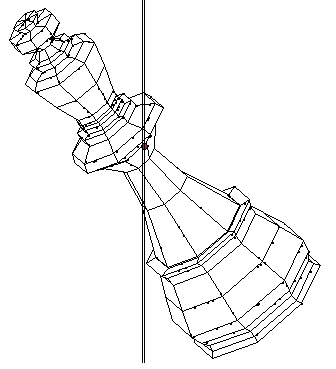
\includegraphics[scale=0.3]{images/king}
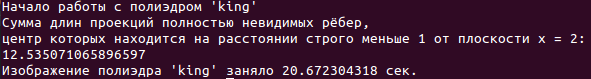
\includegraphics[scale=0.5]{images/king_ex}
\end{center}
\vspace*{-8mm}
\caption{}\label{fig:king}
\end{figure}
